\documentclass{beamer}
\usepackage{graphicx}
\usepackage{listings}
\lstset{
basicstyle=\small\ttfamily,
columns=flexible,
breaklines=true
}
\usepackage{url}
\usepackage[colorinlistoftodos]{todonotes}
%Information to be included in the title page:
\title{Haskell or How I Learned to Stop Worrying and Love in General: Haskell for Flow Cytometry}
\author{Noah Thomas Jones}
\institute{University of Florida}
\date{}
\begin{document}
\frame{\titlepage}
\begin{frame}
  \frametitle{What is Flow?}
  \begin{figure}
    \centering
    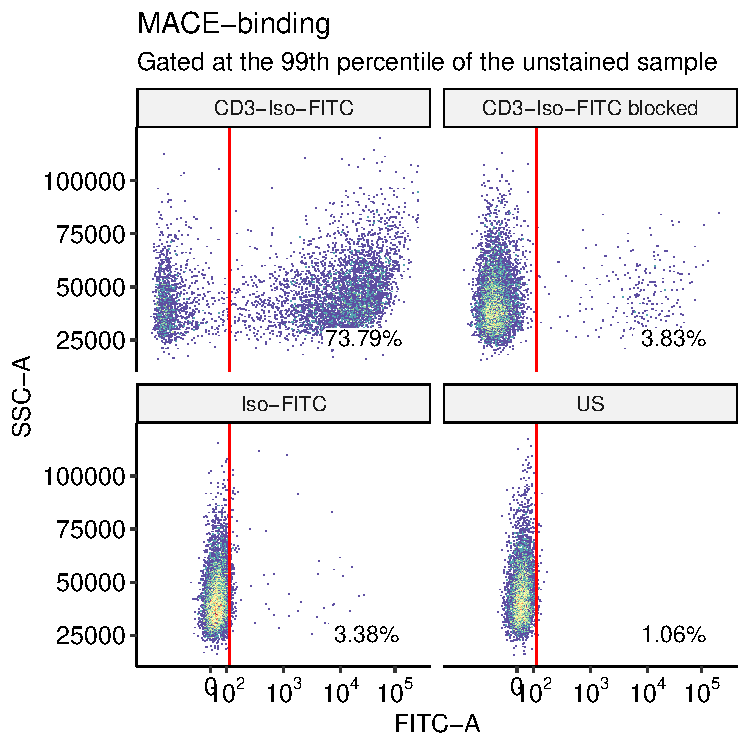
\includegraphics[width=0.45\textwidth]{./images/NJ030_MACE-binding.pdf}
    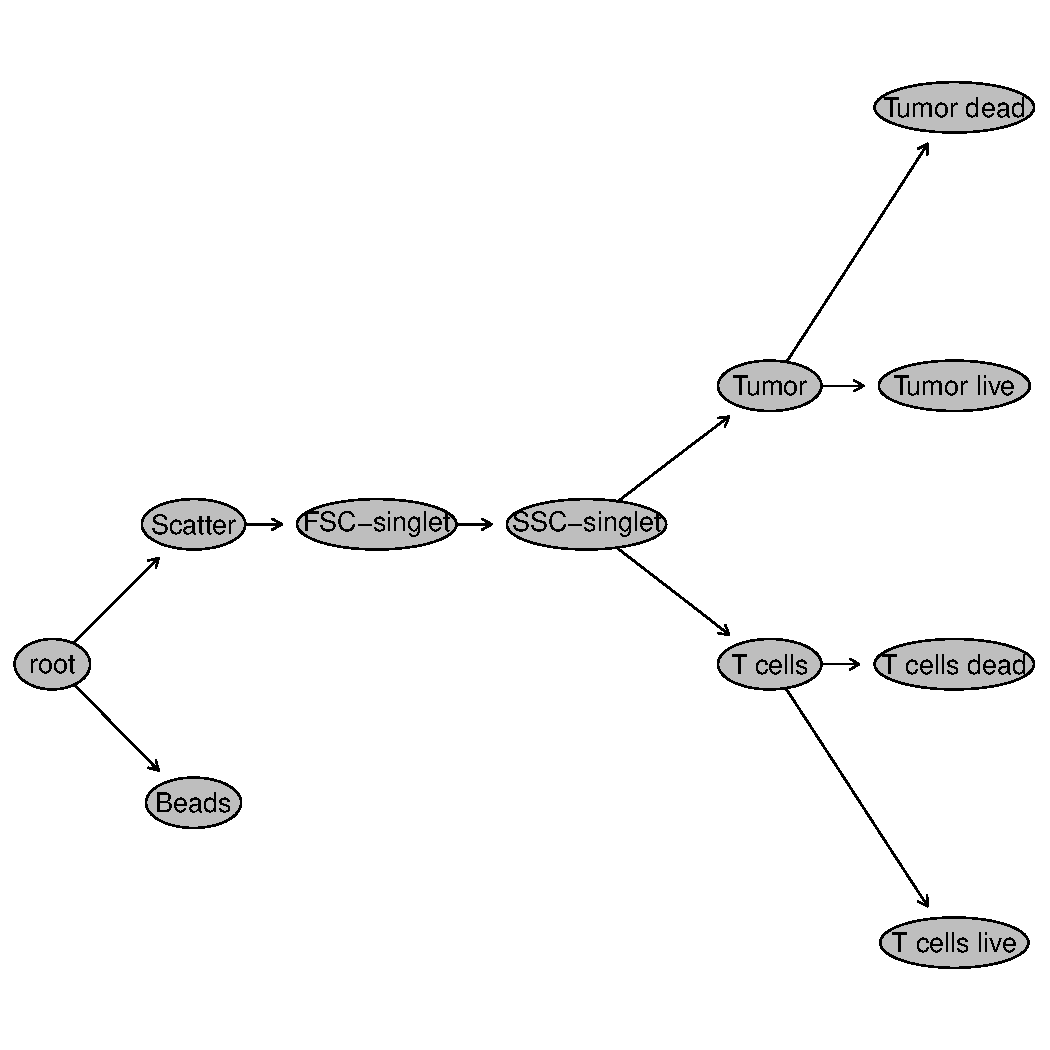
\includegraphics[width=0.45\textwidth]{./images/NJ017_gates.pdf}
    \caption{Examples: gates on fluorescent channels and
      example gating scheme.}
  \end{figure}
\end{frame}
\begin{frame}
  \frametitle{Problem Statement}
  We need flow cytometry gating scheme that does not
\end{frame}
\begin{frame}[fragile]
  \frametitle{Existing Solutions} We have a gating ML
  standard\cite{spidlen2015isac}, which does something for portability
  of gates, but of the tools used, one notable example is the R
  library \texttt{flowCore}, which after defining a \texttt{gatingset} object,
  which is an object tenuously linked to a \texttt{flowset} object, is
  modified through imperative side-effects.
\begin{lstlisting}
rg1 <- rectangleGate("FSC-A"=c(50000, Inf), filterId="NonDebris")
gs_pop_add(gs, rg1, parent = "root")
## [1] 2
gs_get_pop_paths(gs)
## [1] "root" "/NonDebris"
# gate the data
recompute(gs)
## done!
\end{lstlisting}
\end{frame}

\begin{frame}[fragile]
  \frametitle{Getting Started} The first objective was to write a file
  parser so that we can pull data out of our files. We can start based
  on our file specification\cite{spidlen2021data} example:
\begin{lstlisting}
FCS3.0         256    1545    1792  202456       0       0 
\end{lstlisting}
\begin{quotation}
  The primary purpose of the HEADER segment is to describe the location
of the other segments in the data set. The HEADER segment begins at
byte offset zero from the beginning of the data set.  The first six
bytes in the HEADER segment comprise the version identifier
(FCS3.1). Note that there is no space character between the FCS and
the 3.1 in the identifier. The next 4 bytes (6 - 9) are occupied by
space characters (ASCII 32). Following the identifier are at least
three pairs of ASCII-encoded integers indicating the byte offsets for
the start and end (=last byte of) of the primary TEXT segment, the
DATA segment, and the ANALYSIS segment, respectively.
\end{quotation}
\cite{parks2008data}
\end{frame}

\begin{frame}[fragile]
  \frametitle{Example}
  This function does a thing, and here we compare it to alternative package that uses GatingML
\begin{lstlisting}
A proper implementation of GatingML
    \end{lstlisting}
\end{frame}

\nocite{*}
\bibliographystyle{IEEEannot}
\bibliography{bibliography}

\end{document}
